\chapter{INTERFACE IMPLEMENTATION}
\label{chap:GUI_impl.tex}
As tracing the execution log files manually is a time consuming problem, a user friendly interface can help the verification engineer reduce his efforts. A Graphical User Interface will have visual features to select/compare/navigate through log information. The main function of the GUI is to collect and represent related information from different sources for easy access. 

\section {INTERFACE IMPLEMENTATION}
\addtocontents{toc}{\protect\setcounter{tocdepth}{2}}
%\figurename{} 
\begin{figure}[H]
\centering
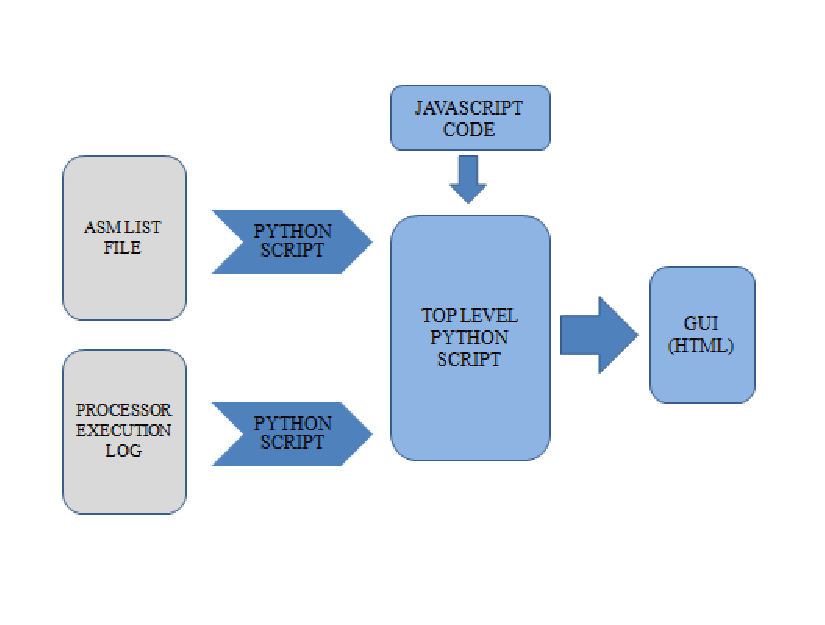
\includegraphics[width=5.5in]{./figures/gui_impl.eps}
\caption{GUI Implementation} 
\label{fig:gui_impl.eps}
\end{figure}

 All relevant processor execution log information and asm test details are provided to the user through a web interface. The interface uses data visualization JavaScript features to develop graphical representation of the log information.
~\figurename{~\ref{fig:gui_impl.eps}}shows the flow of GUI implementation. The log file contents and asm file information are extracted and formatted by using a Python script. JavaScript for the web interface is developed which will have dynamic interactive features for navigating through data. A master Python script will process the data extracted from log files, reads the web design from a JavaScript and generate a single output HTML web page which is the final GUI. Major implementation steps are detailed below.


\subsection {EXTRACTING ASM FILE INFORMATION}
A 64-bit assembler assembles asm test file, configuration file (that define the random operands, segmentation, gdt, ldt, page tables, etc,) and the include files together to generate an assembly list file [1].
%\figurename{} 
%\figurename{} 
\begin{figure}[H]
\centering
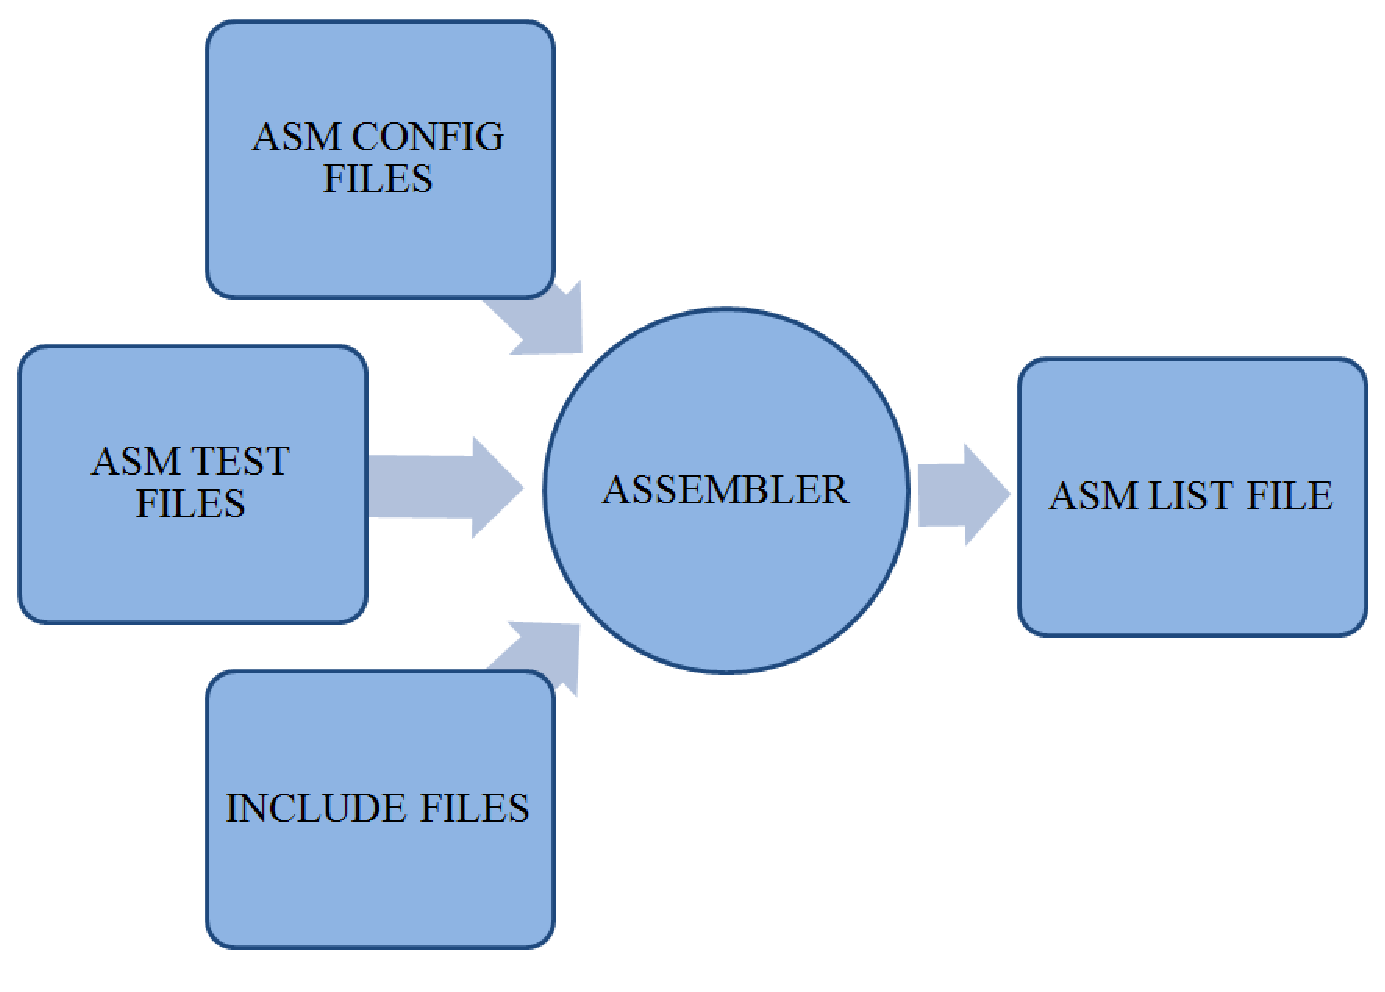
\includegraphics[width=3.5in]{./figures/asm.eps}
\caption{Assembler}
\end{figure}

List file holds details of instructions; opcodes and operand, linear address, module/register configuration details etc. This information are relevant for debugging.
%\figurename{} 
%\figurename{} 
\begin{figure}[H]
\centering
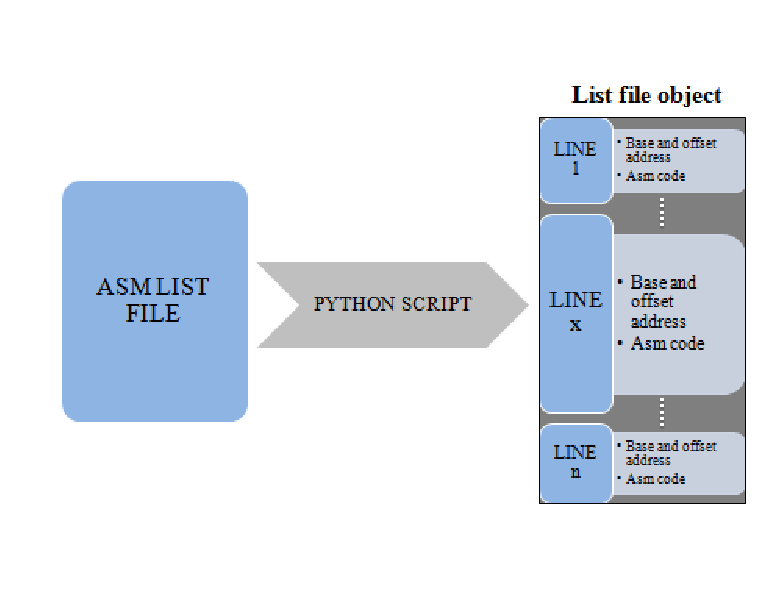
\includegraphics[width=4.5in]{./figures/list.eps}
\caption{Asm List File Extraction}
\end{figure}
A python script extracts the following information from the list file:

\begin{itemize}
	\item[-] Base and offset address value
	\item[-] Instruction line number
	\item[-] The assembly code
\end{itemize}


\subsection {EXTRACTING EXECUTION LOG INFORMATION}
The details of Instruction Level Simulator execution are available in the execution log fie. Debugging require detail traversal through this log file as it holds instruction by instruction execution details which include register states, thread details, flags information etc and other data which help in tracing out the cause of failure. From the log file, a second python program will extract the following information regarding each cycle:

\begin{itemize}
 \item[-] Thread number
 \item[-]  Mode of operation
 \item[-]  Cycle number
 \item[-]  Linear address
 \item[-]  Memory write, Memory read, I/O write/read, Code read
 \item[-]  Branch target (linear address)
 \item[-]  Registers updated with new value
\end{itemize}


\subsection {ADDRESS MAPPING}

In the master python script, the list file information is combined with the execution log information. This is based on mapping the linear address values. As x86 architecture follows segmented memory model along with paging, address translation is required for generating the linear/physical address [2].
\\
\centerline{Linear address = Base address + Offset value}
\\
From the base and offset values extracted from the list file, the linear address is generated and compared with the linear address in the execution log details.


\subsection {DEVELOP THE INTERFACE}

The final step is developing the interface. As the GUI is web based, layout design is done using HTML (Hyper Text Markup Language). However for providing interactive features to the user a much more powerful language is need along with HTML and we use JavaScript.

\emph {\bf JavaScript (JS)} is an interpreted computer programming language. It is  implemented as part of web browsers so that client-side scripts could interact with the user, control the browser, communicate asynchronously, and alter the document content that was displayed. It is a multi-paradigm language, supporting object-oriented, imperative, and functional programming styles.

In addition a style sheet language called CSS (Cascading Style Sheets) is used for describing the presentation semantics (the look and formatting) of the interface page written in HTML.

